\documentclass{beamer}


\title{kubernetes}
\author{Joris Baiutti}
\institute{Berner Fachhochschule}
\date{\today}

\begin{document}
\begin{frame}
\titlepage
\end{frame}

\section{Containers and kubernetes}

\begin{frame}
\frametitle{Why containers}
\begin{itemize}
    \item Isolate applications
    \item Automated deployment
    \item Consistent environment 
    \item todo .....
\end{itemize}
\end{frame}

\begin{frame}
\frametitle{kubernetes, what is it and why we need it}
    \begin{itemize}
        \item abstraction of infrastructure
        \item desired state
        \item automation
    \end{itemize}
\end{frame}

\begin{frame}
\frametitle{What is a pod}
    \begin{figure}
        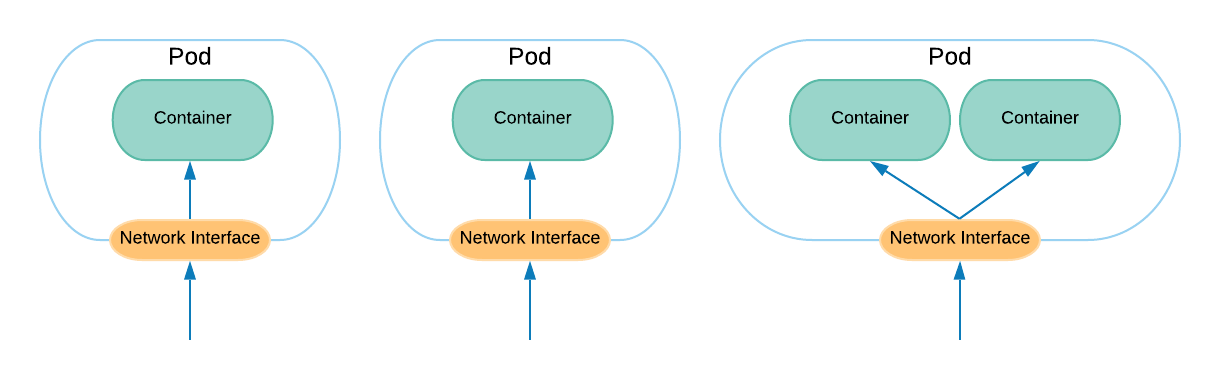
\includegraphics[width=\linewidth]{images/Pods.png}
    \end{figure}
\end{frame}

\begin{frame}
    \frametitle{Using Columns}
    \begin{columns}
    \column{0.5\textwidth}
    Laöoidfnasoidfnasdfn 
    a^dfk
    \column{0.5\textwidth}
    aosidfasif aspdfisd
    \end{columns}
\end{frame}

\begin{frame}
\frametitle{Overview of kubernetes}
\begin{figure}
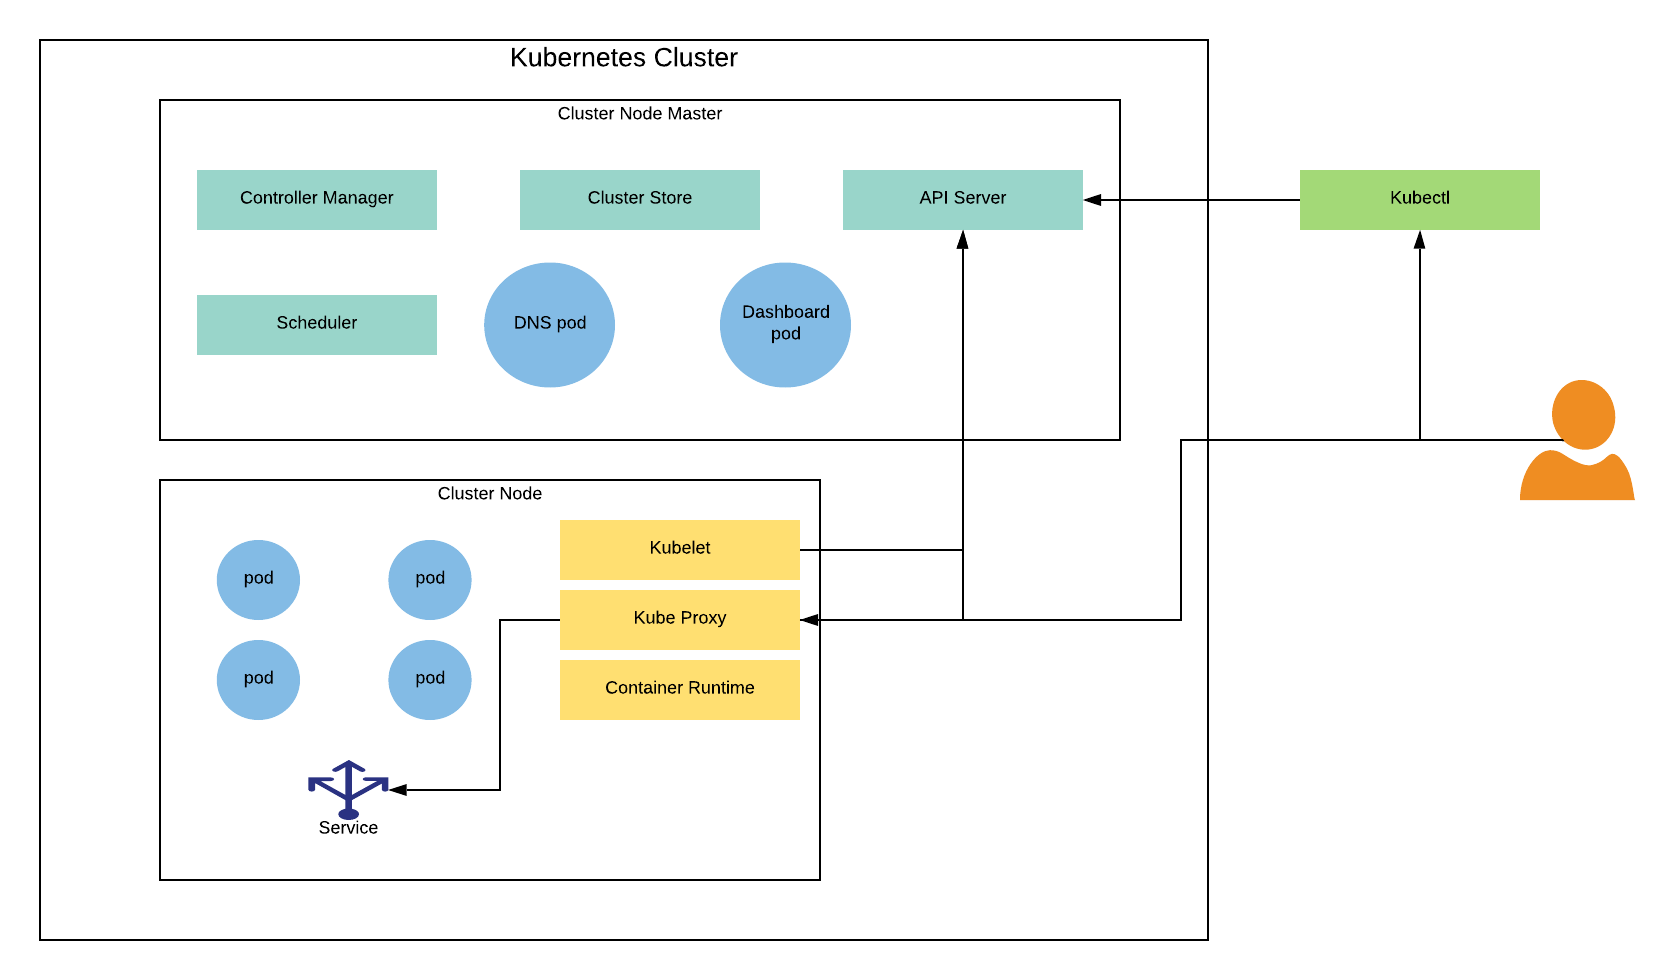
\includegraphics[width=\linewidth]{images/KubernetesOverview.png}
\end{figure}

\end{frame}

\end{document}